\documentclass{beamer}
\usepackage{hyperref}
\usetheme{CambridgeUS}

\title{Linux, vim, and git Workshop}
\subtitle{A Sequence of (Very) Brief Introductions}
\author{Slides: \hyperlink{igithub.com/jleightcap/LinuxVimWorkshop}{github.com/jleightcap/LinuxVimWorkshop}}
\institute{Wireless Club -- Jack Leightcap}
\date{February 3, 2020}

\begin{document}
\begin{frame}
  \titlepage
\end{frame}

\begin{frame}
  \frametitle{Workshop Structure}
  \begin{itemize}
    \item ~15 Minutes -- Linux
    \item ~15 Minutes -- vim
    \item ~30 Minutes -- git
    \item We have the room booked until 8:30, if you want to delve into anything in more depth, we'd love to stick around!
  \end{itemize}
\end{frame}

\begin{frame}
  \frametitle{What is Linux?}
  \begin{itemize}
    \item An open source, cross-platform  Operating System
      \begin{itemize}
        \item Linux distributions are completely free to download and use indefinitely
        \item Culture of making source code publicly available, if something is broken you almost always have the ability to debug it
      \end{itemize}
    \item Could be described as an ecosystem of software
      \begin{itemize}
        \item If you don't like the way some component works, someone probably has already written an alternative
        \item Or you have the complete power to write your own implementation
        \item With most problems there is probably already a thread somewhere online from 2006 about the exact issue you're having
      \end{itemize}
  \end{itemize}
\end{frame}

\begin{frame}
  \frametitle{What is Linux used for, and why should you learn it?}
  \begin{itemize}
    \item A lot here at Northeastern! COE/CCS (sorry, \emph{Khoury}) Linux servers for storage space and remote execution, used heavily in Embedded Design...
    \item A large part of software development takes place using Linux
    \item Embedded Systems programming heavily relies on familiarity with Linux
    \item Devices ranging from Android phones to PS4s all run some modified versions of Unix
    \item Generally most non-desktop processors you can think of run some form of Linux
      \begin{itemize}
        \item Of all processors (micro or not), any guesses what percentage are used in personal computers?
      \end{itemize}
    \item The skills learned in one Linux environment are usually extremely transferable to a wide range of enironments.
  \end{itemize}
\end{frame}

\begin{frame}
  \begin{figure}[ht]
    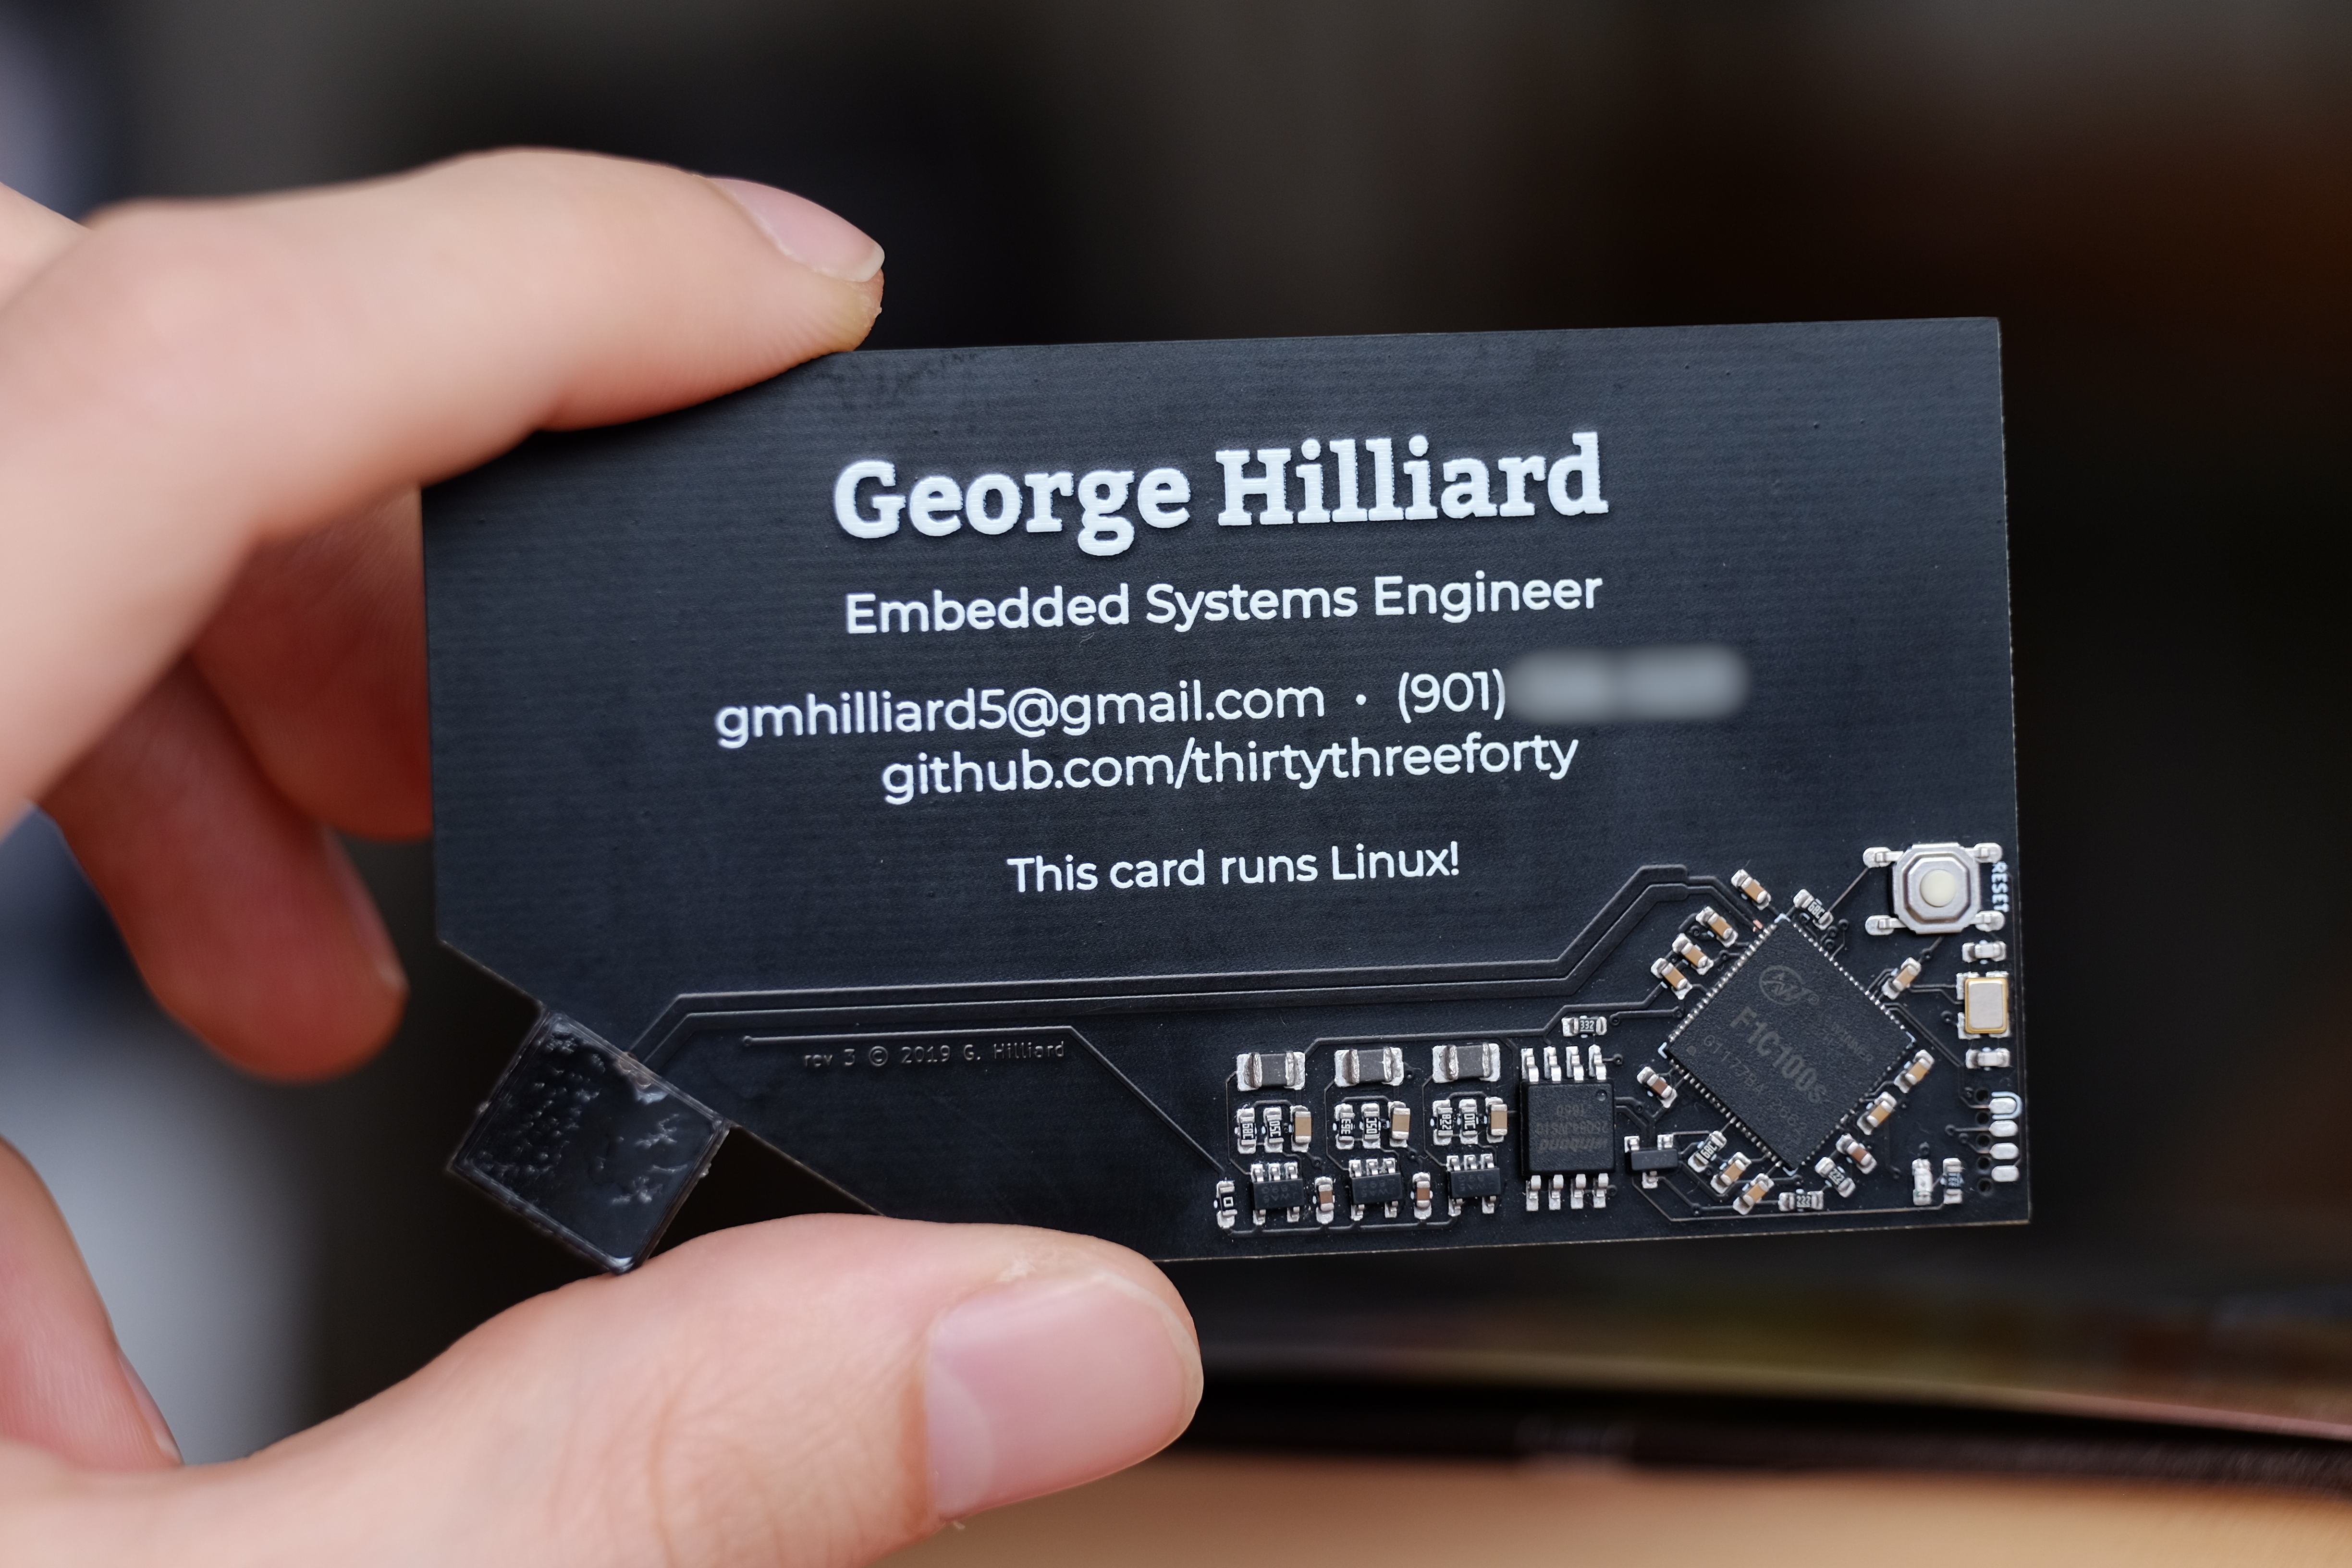
\includegraphics[width=4in]{businesscard-top.jpg}
    \caption{Embedded Linux on business card for \$1.40}
  \end{figure}
\end{frame}

\begin{frame}
  \begin{figure}[ht]
    \includegraphics[width=\textwidth]{tuxserver.jpg}
    \caption{1/3 of Microsoft Azure servers run Linux!}
  \end{figure}
\end{frame}

\begin{frame}
  \frametitle{Linux Basics - The Terminal}
  \begin{columns}[t]
    \begin{column}{.5\textwidth}
      \begin{figure}
        \centering
        \includegraphics[width=\linewidth]{lynx.png}
        \caption{\texttt{Lynx} - a terminal-based browser}
      \end{figure}
    \end{column}
    \begin{column}{.5\textwidth}
      \begin{itemize}
        \item A method of "communicating with your computer" through text-based commands rather than a point-and-click GUI
        \item Can be used for
          \begin{itemize}
            \item Navigating your filesystem
            \item Creating, deleting, or modifying files
            \item Browsing the internet
            \item Checking email
            \item Basically, anything you would use a computer for
          \end{itemize}
        \item You can "live in the terminal"
      \end{itemize}
    \end{column}
  \end{columns}
\end{frame}

\begin{frame}
  \frametitle{Linux Basics -- File Organization 1}
  \begin{columns}[t]
    \begin{column}{.5\textwidth}
      \begin{figure}[h]
        \centering
        \includegraphics[width=\linewidth]{filesystem.png}
        \caption{Basic Linux Directory Structure}
      \end{figure}
    \end{column}
    \begin{column}{.5\textwidth}
      \begin{itemize}
        \item \texttt{cd [directory]}\\
          move your current location to \texttt{directory}
        \item \texttt{mv [source] [destination]}\\
          move a file from \texttt{source} to \texttt{destination}
        \item \texttt{pwd} \\
          print working directory
        \item \texttt{ls} \\
          list the files in the current directory
      \end{itemize}
    \end{column}
  \end{columns}
\end{frame}

\begin{frame}
  \frametitle{Linux Basics -- File Organization 2}
  \begin{columns}
    \begin{column}{.5\textwidth}
      ABSOLUTE PATH
      \begin{itemize}
        \item \texttt{/home/\emph{user}}
        \item The current directory
        \item The parent directory
      \end{itemize}
    \end{column}
    \begin{column}{.5\textwidth}
      RELATIVE PATH
      \begin{itemize}
        \item \texttt{\~}
        \item \texttt{.}
        \item \texttt{..}
      \end{itemize}
    \end{column}
  \end{columns}
  \vspace{1em}
  \begin{center}
    FILE MANIPULATION
  \end{center}
  \vspace{-1em}
  \begin{itemize}
    \item \texttt{touch [file]} -- create an empty file named \texttt{file}
    \item \texttt{rm [file]}  -- remove \texttt{file} (forcibly!)
    \item \texttt{mkdir [directory]} -- make an empty directory named \texttt{directory}
    \item \texttt{rmdir [directory]} -- remove a directory (checks if empty)
    \item \texttt{vim [file]} -- edit a file in vim (foreshadowing?)
  \end{itemize}
\end{frame}

\begin{frame}
  \frametitle{Vim! What is it?}
  \begin{itemize}
    \item Vim is a terminal-based and standalone text editor
    \item Entirely based on keyboard interaction rather than point and click
    \item Hands stay close to the home row of the keyboard throughout text editing
    \item Frequently voted among the most popular text editors among Linux users
  \end{itemize}
  \begin{figure}
    \centering
    \includegraphics[width=0.4\textwidth]{vimspeed.jpg}
  \end{figure}
\end{frame}

\begin{frame}
  \frametitle{Vim Basics -- Modes}
  Vim has different editing modes for different parts of the typing process,
  \begin{itemize}
    \item \emph{Normal Mode} -- the default mode, used for editor commands.
    \item \emph{Visual Mode} -- used to highlight text. Commands executed apply to all highlighted text.
    \item \emph{Insert Mode} -- actually write text from keyboard.
    \item \emph{Command-line Mode} -- execute commands.
  \end{itemize}
  To move between modes,
  \begin{itemize}
    \item Normal mode is the default, at any point press \texttt{esc}.
    \item Visual mode is enabled by pressing \texttt{v} or \texttt{V}.
    \item Insert mode is enabled by pressing \emph{i} (or other shortcut keys)
    \item Command-line Mode is enabled by pressing \texttt{:}
  \end{itemize}
\end{frame}

\begin{frame}
  \frametitle{Vim Basics -- Normal Mode}
  \begin{itemize}
    \item Typing in this mode doesn't actually insert any text!
    \item Some basic movements:
      \begin{itemize}
        \item \texttt{\{h, j, k, l\}} $\rightarrow$ \{left, down, up, right\}
        \item \texttt{w/W} -- move forward by a word (punctuation, whitespace)
        \item \texttt{b/B} -- move backward by same rule as \texttt{w/W} 
        \item \texttt{e/E} -- move forward by same rule as \texttt{w/W}, but to the end of word
        \item \texttt{\^{}/\$} -- the start/end of the current line
        \item \texttt{gg/GG} -- the first/last line of the current file
        \item $n$\texttt{gg} -- go to the $n$th line of the current file
        \item all commands can be prefixed by a number, so \texttt{4k} would move up 4 lines
      \end{itemize}
    \item Some basic editing:
      \begin{itemize}
        \item \texttt{x} -- delete character under cursor
        \item \texttt{diw} - delete in word, delete word under cursor
        \item \texttt{dd} -- delete the current line
      \end{itemize}
  \end{itemize}
\end{frame}

\begin{frame}
  \frametitle{Vim Basics -- Visual Mode}
  Much simpler than insert mode! Define selection start and end, then execute a command over that selection.
  \begin{itemize}
    \item \texttt{v} - start highlighting at current cursor position by character
    \item \texttt{V} - start highlighting at the current line by line
  \end{itemize}
  Visual mode is generally useful for commands repeated over multiple lines.
  \begin{itemize}
    \item \texttt{<</>>} -- indent back/forward
    \item \texttt{d} - delete,  equivalent to "cut" -- move into "clipboard" (buffer in vim)
    \item \texttt{y} -- yank, equivalent to "copy"
    \item \texttt{p} -- paste text in buffer after the cursor
  \end{itemize}
  To repeat a command, prefix with a number as mentioned before, or use \texttt{.}
\end{frame}

\begin{frame}
  \frametitle{Vim Basics -- Insert Mode}
  Actually input text! There's not much to say about this, so some shortcuts that enter insert mode:
  \begin{itemize}
    \item \texttt{a/A} -- append, at end of word/line
    \item \texttt{i/I} - insert, at current cursor position, or at beginning of line
    \item \texttt{ct\{x\}} -- change to \texttt{x}, delete text from cursor position to \texttt{x}, and enter insert mode
    \item \texttt{c\^{}/c\$} -- change to beginning of line, change to end of line
  \end{itemize}
\end{frame}

\begin{frame}
  \frametitle{Vim Basics -- Command-line Mode}
  \begin{columns}
    \begin{column}{.6\textwidth}
  Enter commands after \texttt{:},
  \begin{itemize}
    \item \texttt{:w,:q} -- write, quit 
    \item \texttt{:![command]} -- run terminal \texttt{command} from inside vim!
    \item \texttt{/[string]} -- search for \texttt{string} in current file, \texttt{n/N} to navigate instances
  \end{itemize}
    \end{column}
    \begin{column}{.4\textwidth}
      \includegraphics[width=\linewidth]{vimexit.jpg}
    \end{column}
  \end{columns}
\end{frame}

\begin{frame}
  \frametitle{Actually Trying Vim and Linux!}
  A lecture about Vim is pretty dry, and is something that is learned through practice.\\
  If we have time, some good resources:
  \begin{itemize}
    \item VIM Adventures (vim-adventures.com) -- a browser game that visualizes vim commands very well
    \item \texttt{vimtutor} -- frequently comes installed alongside vim.
    \item Vim Tips Wiki (vim.fandom.com) -- if you end up going down this rabbit hole, as plenty examples of surprisingly efficient commands.
    \item Over the Wire (overthewire.org/wargames/bandit/) -- SSH based game based on finding keys, targeted at Linux beginners.
  \end{itemize}
\end{frame}

\end{document}
